\chapter{MÔ HÌNH HỌC SÂU TRONG PHÁT HIỆN BẤT THƯỜNG}

\section{Giới thiệu bài toán}

Trong kiểm tra chất lượng sản phẩm công nghiệp, các lỗi như vết xước, nứt, biến dạng hoặc thiếu chi tiết có thể xuất hiện với hình dạng và kích thước khác nhau. Việc kiểm tra thủ công phụ thuộc vào kinh nghiệm và khả năng quan sát của người thực hiện. Một hệ thống phân tích ảnh có thể hỗ trợ phát hiện dấu hiệu bất thường và chỉ ra vị trí cần kiểm tra, từ đó giúp quá trình đánh giá chất lượng có thêm căn cứ trực quan.

Khó khăn của bài toán nằm ở sự chênh lệch giữa dữ liệu bình thường và dữ liệu lỗi. Ảnh sản phẩm đạt yêu cầu thường dễ thu thập hơn, trong khi một số dạng lỗi ít xuất hiện hoặc chưa từng được ghi nhận. Nếu xây dựng bộ phân loại có giám sát cho từng loại lỗi, tập huấn luyện phải có đủ ví dụ đại diện của các lỗi đó. Điều kiện này khó đáp ứng khi lỗi mới tiếp tục phát sinh trong quá trình sản xuất.

Đề tài của nhóm 13 nghiên cứu hướng học đặc điểm của sản phẩm bình thường rồi đánh giá mức độ khác biệt của ảnh mới. Tập huấn luyện chỉ sử dụng ảnh tốt; ảnh lỗi và mặt nạ vùng lỗi được dùng ở bước đánh giá. Cách tổ chức này thường được gọi là thiết lập học một lớp, và trong phạm vi đề tài được triển khai theo hướng phát hiện bất thường không giám sát.

Hai nhiệm vụ cần giải quyết là phát hiện bất thường ở mức ảnh và định vị bất thường ở mức điểm ảnh. Nhiệm vụ thứ nhất tạo một điểm số cho toàn bộ ảnh để biểu thị mức độ nghi ngờ có lỗi. Nhiệm vụ thứ hai tạo bản đồ điểm bất thường, trong đó mỗi vị trí có giá trị phản ánh độ khác biệt so với đặc điểm bình thường. Điểm số càng cao thì mức độ bất thường càng lớn; điểm số này không mặc nhiên là xác suất có lỗi.

Chẳng hạn, với ảnh một sản phẩm có vết xước nhỏ, hệ thống cần vừa đánh giá ảnh đó có dấu hiệu lỗi, vừa làm nổi bật vùng vết xước. Một mô hình chỉ trả về nhãn toàn ảnh chưa đủ cho yêu cầu định vị. Ngược lại, một bản đồ có nhiều vùng sáng do nền hoặc ánh sáng thay đổi cũng chưa bảo đảm hệ thống nhận diện đúng lỗi thực tế.

Đối tượng nghiên cứu là bộ dữ liệu MVTec AD với 15 loại đối tượng và bề mặt. Theo giao thức nhóm đã thống nhất, mỗi loại có một mô hình riêng; các phương pháp được so sánh bằng image-AUROC và pixel-AUROC trên cùng tập kiểm thử~\cite{bergmannMVTecADComprehensive2019,nhom13MVTecAnomalyDetection2026}. Chương này trình bày nguyên lý và định hướng lựa chọn phương pháp. Kiến trúc cụ thể, cấu hình chạy và kết quả đo sẽ được bổ sung khi phần triển khai hoàn thành.

\begin{figure}[htbp]
  \centering
  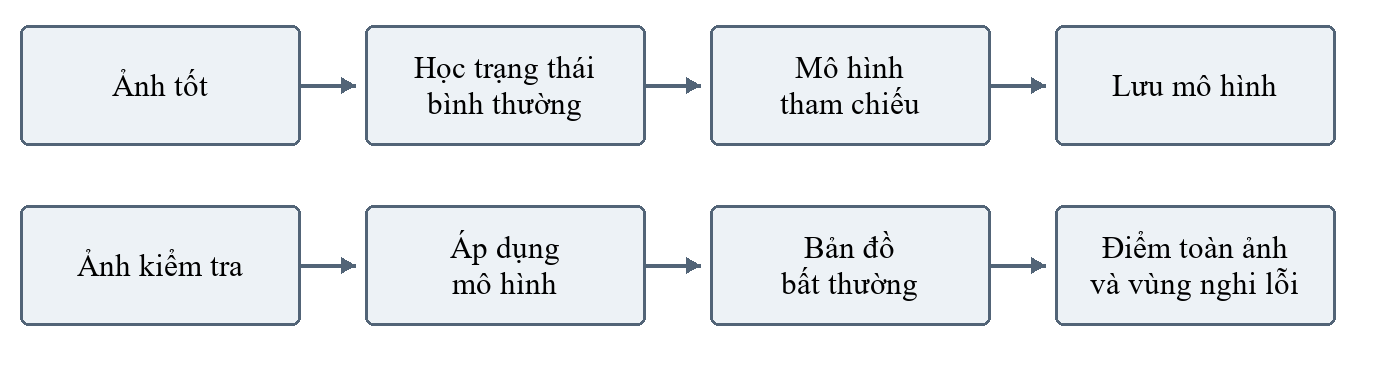
\includegraphics[width=0.9\linewidth]{images/img08.png}
  \caption{Quy trình tổng quát của bài toán phát hiện và định vị bất thường (Sơ đồ nguyên lý, không phải kết quả thực nghiệm)}
  \label{fig:overview}
\end{figure}

\section{Tổng quan các hướng tiếp cận}

\subsection{Phương pháp dựa trên tái tạo ảnh}

Các phương pháp tái tạo học một phép biến đổi để phục hồi đầu vào từ một biểu diễn trung gian. Khi chỉ được học trên ảnh tốt, mô hình được kỳ vọng tái tạo tốt các cấu trúc bình thường. Sự khác biệt giữa ảnh đầu vào và ảnh tái tạo là cơ sở xây dựng điểm bất thường. Autoencoder là mô hình tiêu biểu cho hướng tiếp cận này~\cite{goodfellowDeepLearning2016}.

Ưu điểm của hướng tái tạo là có thể quan sát trực tiếp ảnh đầu vào, ảnh phục hồi và bản đồ sai số. Tuy nhiên, giả thiết ảnh lỗi luôn có sai số tái tạo lớn không phải lúc nào cũng đúng. Mạng có thể tái tạo được cả vùng lỗi hoặc làm mờ các chi tiết bình thường, dẫn đến bỏ sót hoặc cảnh báo nhầm. Vì vậy, chất lượng tái tạo và khả năng phát hiện lỗi phải được đánh giá riêng.

\subsection{Phương pháp dựa trên đặc trưng học trước}

Một mạng nơ-ron tích chập đã được huấn luyện trước có thể được dùng làm bộ trích xuất đặc trưng. Thay vì chỉ so sánh màu sắc tại từng điểm ảnh, hệ thống làm việc với các vector mô tả kết cấu, đường nét và cấu trúc cục bộ. Đầu ra của các tầng trung gian vẫn giữ thông tin không gian, phù hợp với yêu cầu xác định vị trí bất thường.

Trong hướng này, trọng số của bộ trích xuất có thể được giữ cố định. Giai đoạn xây dựng mô hình trên ảnh tốt tập trung vào tính toán thống kê hoặc lưu giữ đặc trưng tham chiếu. Như vậy, việc sử dụng mạng học sâu không đồng nghĩa với việc phải huấn luyện lại toàn bộ mạng trên dữ liệu của đề tài. PaDiM và PatchCore là hai phương pháp nhóm dự kiến nghiên cứu theo hướng này~\cite{defardPaDiMPatchDistribution2021,rothTotalRecallIndustrial2022,nhom13MVTecAnomalyDetection2026}.

PaDiM mô hình hóa sự biến thiên của đặc trưng tại từng vị trí bằng các tham số thống kê. PatchCore lưu một tập đặc trưng bình thường đại diện rồi đối chiếu đặc trưng ảnh mới với tập đó. Hai cách biểu diễn này tạo ra những yêu cầu khác nhau về bộ nhớ, phép tính suy luận và mức độ phụ thuộc vào vị trí của vật thể.

\subsection{Phạm vi các phương pháp được lựa chọn}

Nhóm lựa chọn Autoencoder làm mô hình cơ sở để khảo sát hướng tái tạo; PaDiM và PatchCore là hai phương pháp chính để khảo sát hướng sử dụng đặc trưng học trước. Sự lựa chọn này cho phép đối chiếu ba cách biểu diễn trạng thái bình thường: trọng số của mạng tái tạo, phân phối thống kê và tập vector tham chiếu.

Việc so sánh không chỉ nhằm tìm phương pháp có AUROC cao hơn. Nhóm còn cần xem xét dạng lỗi bị bỏ sót, vùng cảnh báo nhầm và chi phí tài nguyên. Một phương pháp có chất lượng tốt trên bề mặt ít biến động chưa chắc giữ được ưu thế trên sản phẩm có tư thế thay đổi. Các nhận định về ưu thế thực tế chỉ được kết luận sau khi có kết quả trên dữ liệu của nhóm.

\section{Các mô hình và phương pháp sử dụng}

\subsection{Mô hình Autoencoder}

Autoencoder gồm bộ mã hóa và bộ giải mã. Bộ mã hóa chuyển ảnh đầu vào thành biểu diễn tiềm ẩn; bộ giải mã sử dụng biểu diễn đó để tái tạo ảnh. Với ảnh $x$, ký hiệu $f$ là bộ mã hóa, $g$ là bộ giải mã và $z$ là biểu diễn trung gian, quá trình truyền tiến có dạng~\cite{goodfellowDeepLearning2016}:
\begin{equation}
  z = f(x), \qquad \hat{x} = g(z) = g\bigl(f(x)\bigr)
  \label{eq:ae-forward}
\end{equation}

Đối với ảnh công nghiệp, một Autoencoder tích chập là hướng triển khai phù hợp để khai thác quan hệ lân cận giữa các điểm ảnh. Các lớp mã hóa giảm kích thước không gian và xây dựng đặc trưng; các lớp giải mã khôi phục kích thước đầu ra. Biểu diễn ở phần cổ chai giới hạn lượng thông tin truyền qua, buộc mô hình chọn lọc các cấu trúc cần thiết để phục hồi ảnh.

\begin{figure}[htbp]
  \centering
  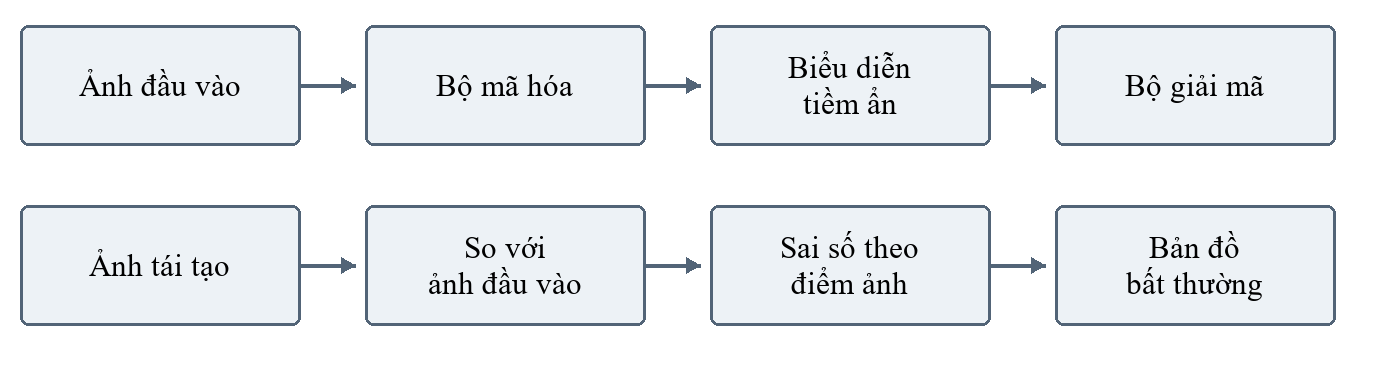
\includegraphics[width=0.9\linewidth]{images/img09.png}
  \caption{Nguyên lý tái tạo và tính bản đồ sai số của Autoencoder (Sơ đồ nguyên lý, không phải kết quả thực nghiệm)}
  \label{fig:ae}
\end{figure}

Một hàm mất mát khởi đầu có thể sử dụng là sai số bình phương trung bình. Với ảnh có chiều cao $H$, chiều rộng $W$ và $C$ kênh, mất mát tái tạo được viết như sau:
\begin{equation}
  L(x,\hat{x}) = \frac{1}{HWC}\sum_{u=1}^{H}\sum_{v=1}^{W}\sum_{c=1}^{C}
  \bigl[x(u,v,c) - \hat{x}(u,v,c)\bigr]^{2}
  \label{eq:ae-loss}
\end{equation}

Các tổng được lấy trên toàn bộ vị trí và kênh ảnh. Trong huấn luyện, giá trị mất mát được trung bình trên các mẫu trong lô dữ liệu; thuật toán tối ưu cập nhật trọng số để giảm sai số. Đầu vào và ảnh tái tạo phải có cùng kích thước và cùng thang giá trị thì phép so sánh mới có ý nghĩa.

Ở bước kiểm tra, sai số tại mỗi vị trí có thể được lấy trung bình theo các kênh màu để tạo bản đồ $A(u,v)$. Sau bước làm mượt nếu có, một cách tổng hợp đơn giản là lấy giá trị lớn nhất của bản đồ làm điểm bất thường của ảnh. Cách tổng hợp này nhạy với lỗi cục bộ, nhưng cũng có thể bị ảnh hưởng bởi một vài vị trí nhiễu có sai số cao.
\begin{equation}
  A(u,v) = \frac{1}{C}\sum_{c=1}^{C}\bigl[x(u,v,c) - \hat{x}(u,v,c)\bigr]^{2}
  \label{eq:ae-map}
\end{equation}

Kích thước cổ chai là một yếu tố cần khảo sát. Cổ chai quá nhỏ có thể làm mất các kết cấu bình thường; mạng có năng lực quá lớn lại có khả năng phục hồi cả chi tiết lỗi. Ngoài ra, sai số ở mức điểm ảnh dễ thay đổi theo điều kiện chiếu sáng và chất lượng ảnh. Đây là các giả thuyết cần đối chiếu bằng ảnh tái tạo và bản đồ bất thường, không phải kết quả đã được xác nhận trong đề tài.

Trong kế hoạch hiện tại, nhóm dự kiến tự xây dựng Autoencoder làm mốc so sánh. Số lớp, số kênh, kích thước biểu diễn tiềm ẩn, hàm mất mát, số epoch và tốc độ học chưa được xem là cấu hình cuối cùng. Các giá trị gợi ý trong kho mã nguồn chỉ là điểm xuất phát cho việc triển khai~\cite{nhom13MVTecAnomalyDetection2026}.

\subsection{Phương pháp PaDiM}

PaDiM, viết tắt của Patch Distribution Modeling, sử dụng đặc trưng từ CNN học trước để mô tả các vùng cục bộ của ảnh. Các đặc trưng ở nhiều tầng được đưa về lưới không gian tương ứng rồi ghép lại. Việc kết hợp các tầng cho phép biểu diễn chứa thông tin ở nhiều mức độ chi tiết~\cite{defardPaDiMPatchDistribution2021}.

Theo định hướng trong tài liệu dự án, bộ trích xuất được giữ cố định. Tại mỗi vị trí của lưới đặc trưng, nhóm thu các vector từ ảnh tốt, lựa chọn một tập chiều đặc trưng và ước lượng trung bình cùng ma trận hiệp phương sai. Các chỉ số chiều được chọn phải thống nhất giữa bước xây dựng mô hình và bước kiểm tra~\cite{nhom13MVTecAnomalyDetection2026}.

\begin{figure}[htbp]
  \centering
  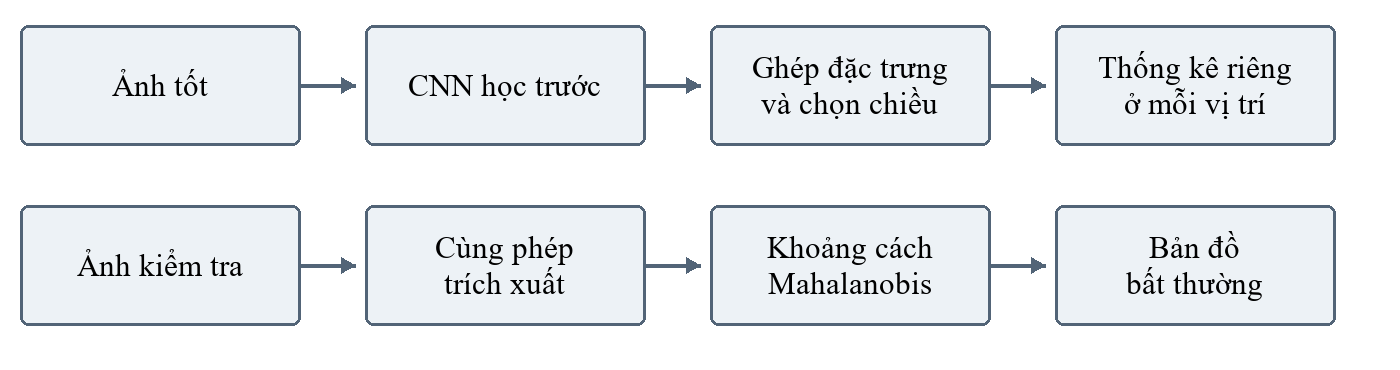
\includegraphics[width=0.9\linewidth]{images/img10.png}
  \caption{Luồng xử lý của PaDiM với thống kê riêng theo vị trí (Sơ đồ nguyên lý, không phải kết quả thực nghiệm)}
  \label{fig:padim}
\end{figure}

Gọi $z_k(p)$ là vector đặc trưng của ảnh huấn luyện thứ $k$ tại vị trí $p$; $N$ là số ảnh tốt. Các công thức thống kê mẫu được sử dụng để mô tả tập vector tại vị trí đó:
\begin{align}
  \mu_p &= \frac{1}{N}\sum_{k=1}^{N} z_k(p) \label{eq:padim-mean}\\
  \Sigma_p &= \frac{1}{N-1}\sum_{k=1}^{N}\bigl[z_k(p)-\mu_p\bigr]\bigl[z_k(p)-\mu_p\bigr]^{\top} + \varepsilon I \label{eq:padim-cov}
\end{align}

Trong đó $I$ là ma trận đơn vị và $\varepsilon$ là một số dương nhỏ. Thành phần $\varepsilon I$ hỗ trợ ổn định phép tính khi ma trận hiệp phương sai gần suy biến, đặc biệt khi số chiều đặc trưng lớn so với số mẫu. Giá trị $\varepsilon$ là một tham số triển khai cần được ghi lại để tái lập kết quả.

Với vector $z(p)$ của ảnh kiểm tra, khoảng cách Mahalanobis tới thống kê bình thường được dùng làm điểm bất thường tại vị trí $p$:
\begin{equation}
  d_p = \sqrt{\bigl[z(p)-\mu_p\bigr]^{\top}\,\Sigma_p^{-1}\,\bigl[z(p)-\mu_p\bigr]}
  \label{eq:padim-mahalanobis}
\end{equation}

Khác với khoảng cách Euclid thuần túy, biểu thức này có xét đến độ biến thiên và tương quan giữa các chiều. Một sai lệch trên chiều đặc trưng vốn ổn định có thể đáng chú ý hơn một sai lệch cùng độ lớn trên chiều thường xuyên biến động. Các điểm $d_p$ được sắp về lưới không gian và nội suy để tạo bản đồ bất thường ở kích thước đánh giá.

Điểm cần lưu ý trong kế hoạch triển khai là PaDiM lưu thống kê riêng cho từng vị trí. Khi vật thể dịch chuyển hoặc xoay, cùng một vị trí có thể nhận các cấu trúc khác nhau giữa những ảnh tốt. Nhóm cần kiểm tra ảnh hưởng này trên các loại sản phẩm thích hợp. Bộ nhớ lưu ma trận cũng tăng nhanh khi tăng số chiều; vì vậy lựa chọn số chiều phải cân nhắc cùng độ phân giải của lưới đặc trưng~\cite{nhom13MVTecAnomalyDetection2026}.

ResNet18, các tầng trích xuất và số chiều đặc trưng trong tài liệu dự án hiện mới mang tính gợi ý. Báo cáo sẽ ghi đúng backbone, tầng, phép giảm chiều và tham số ổn định hóa sau khi nhóm lựa chọn và chạy thực nghiệm.

\subsection{Phương pháp PatchCore}

PatchCore biểu diễn trạng thái bình thường bằng một bộ nhớ chứa các vector đặc trưng cục bộ đại diện. Phương pháp sử dụng CNN học trước, tổng hợp đặc trưng vùng lân cận và chọn một tập con đại diện để giảm lượng dữ liệu cần lưu. Khi kiểm tra, đặc trưng mới được so với các vector gần nhất trong bộ nhớ~\cite{rothTotalRecallIndustrial2022}.

Theo phương án nghiên cứu của nhóm, giai đoạn xây dựng bộ nhớ bắt đầu từ ảnh tốt của từng loại sản phẩm. Sau khi trích xuất đặc trưng, các vector cục bộ được tập hợp vào một tập chung. Khác với việc lập một phân phối riêng cho từng tọa độ, phép tra cứu sử dụng các mẫu tham chiếu trong bộ nhớ mà không buộc vector phải đến từ đúng vị trí ảnh ban đầu~\cite{nhom13MVTecAnomalyDetection2026}.

\begin{figure}[htbp]
  \centering
  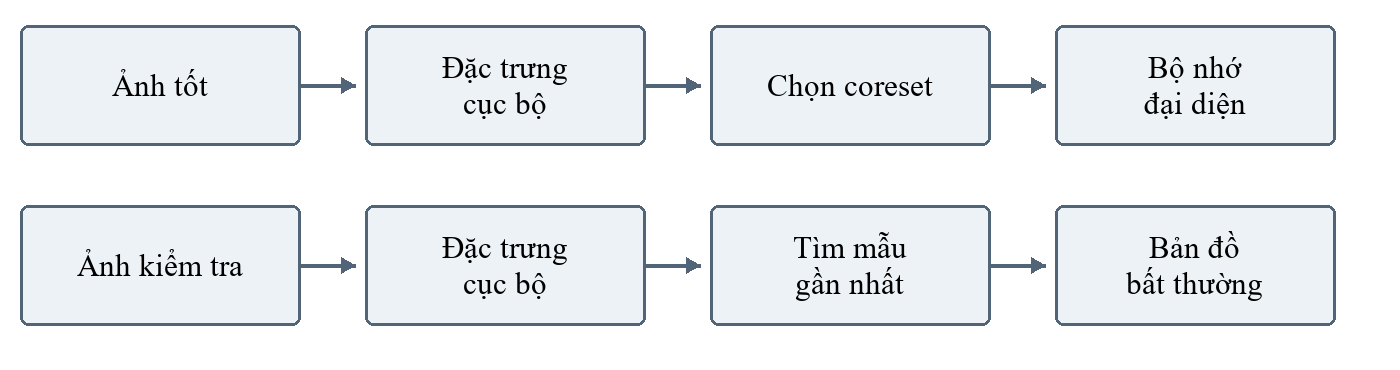
\includegraphics[width=0.9\linewidth]{images/img11.png}
  \caption{Nguyên lý xây dựng bộ nhớ và tra cứu của PatchCore (Sơ đồ nguyên lý, không phải kết quả thực nghiệm)}
  \label{fig:patchcore}
\end{figure}

Lưu toàn bộ vector có thể tạo ra nhiều mẫu gần giống nhau. Bước chọn tập con đại diện, gọi là coreset, nhằm giảm sự dư thừa trong khi vẫn giữ độ bao phủ của không gian đặc trưng. Tỷ lệ giữ lại là một yếu tố cần khảo sát: tập quá nhỏ có thể bỏ mất biến thiên bình thường, còn tập lớn tăng chi phí lưu trữ và tìm kiếm.

Gọi $M$ là tập vector đã được chọn và $q$ là vector của một vùng trong ảnh kiểm tra. Điểm bất thường cục bộ cơ bản có thể được diễn giải bằng khoảng cách tới mẫu gần nhất:
\begin{equation}
  a(q) = \min_{m \in M}\,\lVert q - m\rVert_{2}
  \label{eq:patchcore-score}
\end{equation}

Nếu $q$ ở xa các vector bình thường được lưu, vùng đó nhận điểm cao. Sau khi tính cho các vị trí, các điểm được đưa về lưới ảnh để tạo bản đồ bất thường. Công thức trên mô tả điểm cục bộ; cách tạo điểm cho toàn ảnh còn tùy phiên bản triển khai. Bài báo PatchCore có bước điều chỉnh trọng số khi tính điểm ảnh, nên không nên mặc nhiên coi mọi bản dùng giá trị cực đại đơn giản là tái hiện đầy đủ phương pháp gốc~\cite{rothTotalRecallIndustrial2022}.

Trong đề tài, nhóm cần ghi rõ cách tính điểm ảnh khi sử dụng thư viện hoặc tự cài đặt. Giao thức chung cho phép mỗi phương pháp tạo điểm ảnh của mình; khi không có cách riêng, hàm đánh giá chung sử dụng giá trị lớn nhất của bản đồ đã làm mượt. Mọi thay đổi về cách tổng hợp phải được lưu cùng cấu hình chạy~\cite{nhom13MVTecAnomalyDetection2026}.

Việc bỏ ràng buộc khớp đúng vị trí tạo cơ hội nhận diện các vùng bình thường khi vật thể thay đổi tư thế, nhưng không bảo đảm bất biến với mọi phép xoay hoặc dịch chuyển. Kết quả vẫn phụ thuộc vào đặc trưng học trước và mức độ bao phủ của bộ nhớ. Những lỗi về quan hệ giữa các bộ phận cũng cần được phân tích, vì từng vùng nhỏ có thể vẫn giống mẫu bình thường dù bố cục tổng thể đã sai.

Trong kế hoạch phân công, hai thành viên cùng thực hiện PatchCore trên các nhóm loại sản phẩm khác nhau. Vì vậy, backbone, tầng trích xuất, tỷ lệ coreset, seed và cách tính điểm phải thống nhất trước khi tổng hợp kết quả. Cấu hình gợi ý hiện có trong kho mã nguồn chưa phải cấu hình thực nghiệm đã chốt~\cite{nhom13MVTecAnomalyDetection2026}.

\section{Lý do lựa chọn các phương pháp cho đề tài}

Ba phương pháp được lựa chọn cùng đáp ứng điều kiện xây dựng mô hình từ ảnh tốt và có khả năng tạo bản đồ bất thường. Autoencoder giúp nhóm thực hành thiết kế mạng, lan truyền ngược và tối ưu tham số. PaDiM bổ sung cách tiếp cận thống kê trên đặc trưng học sâu, còn PatchCore cho phép khảo sát cách lưu giữ và tìm kiếm các mẫu đặc trưng đại diện.

Về nội dung học phần, bộ phương pháp này liên kết kiến thức mạng nơ-ron, biểu diễn đặc trưng, đại số tuyến tính và đánh giá mô hình với một bài toán thống nhất. Về thực nghiệm, chúng tạo điều kiện phân tích sự đánh đổi giữa chất lượng phát hiện, bộ nhớ và thời gian suy luận. Bảng~\ref{tab:compare} tổng hợp khác biệt về nguyên lý; bảng không biểu thị thứ hạng hiệu năng của các mô hình do nhóm triển khai.

\begin{table}[htbp]
  \centering
  \caption{So sánh nguyên lý của ba phương pháp}
  \label{tab:compare}
  \small
  \begin{tabular}{@{}>{\raggedright\arraybackslash}p{3cm} >{\raggedright\arraybackslash}p{3.2cm} >{\raggedright\arraybackslash}p{3.7cm} >{\raggedright\arraybackslash}p{3.7cm}@{}}
    \toprule
    Tiêu chí & Autoencoder & PaDiM & PatchCore \\
    \midrule
    Biểu diễn bình thường & Trọng số mạng tái tạo & Trung bình, hiệp phương sai theo vị trí & Tập vector đặc trưng đại diện \\
    Bước xây dựng & Tối ưu trọng số mạng & Trích xuất và tính thống kê & Trích xuất và chọn coreset \\
    Điểm cục bộ & Sai số tái tạo & Khoảng cách Mahalanobis & Khoảng cách tới mẫu gần nhất \\
    Điểm cần khảo sát & Tái tạo mờ hoặc tái tạo cả lỗi & Phụ thuộc vị trí và số chiều & Kích thước bộ nhớ và chi phí tìm kiếm \\
    \bottomrule
  \end{tabular}
\end{table}

Không có căn cứ để khẳng định trước một phương pháp luôn tốt hơn hai phương pháp còn lại trên mọi loại sản phẩm. Nhóm dự kiến xem xét cả kết quả trung bình và kết quả riêng từng loại, đồng thời đối chiếu ảnh gốc, mặt nạ chuẩn và bản đồ dự đoán. Cách phân tích này giúp phân biệt lỗi bỏ sót, cảnh báo nhầm trên nền và trường hợp xác định đúng ảnh có lỗi nhưng khoanh vùng chưa chính xác.

\section{Định hướng triển khai và đánh giá}

Theo giao thức trong kho mã nguồn, mỗi phương pháp được xây dựng riêng cho từng loại của MVTec AD, chỉ sử dụng thư mục \texttt{train/good} trong giai đoạn học trạng thái bình thường. Tập test được giữ cho đánh giá cuối cùng; nhóm không điều chỉnh siêu tham số dựa trên kết quả của tập này. Nếu cần xác thực trong quá trình phát triển, cách tách dữ liệu phải được mô tả và bảo đảm độc lập với tập kiểm thử~\cite{nhom13MVTecAnomalyDetection2026}.

Bản đồ bất thường đưa vào bộ đánh giá có kích thước $256 \times 256$ và phải khớp tọa độ với mặt nạ chuẩn. Khi đổi kích thước mặt nạ nhị phân, nhóm sử dụng nội suy lân cận gần nhất để giữ nhãn 0/1. Độ phân giải bên trong mô hình có thể khác, nhưng bước chuyển đổi về kích thước đánh giá phải được thực hiện nhất quán. Thứ tự ảnh, nhãn, mặt nạ và bản đồ dự đoán cũng phải trùng nhau.

Image-AUROC được tính từ điểm toàn ảnh và nhãn tốt hoặc lỗi; pixel-AUROC được tính từ điểm tại các pixel và mặt nạ vùng lỗi. AUROC đánh giá khả năng xếp hạng khi thay đổi ngưỡng, không yêu cầu chọn trước một ngưỡng phân loại duy nhất~\cite{scikit-learnRocAucScore}. Các chỉ số được tính riêng từng loại rồi lấy trung bình theo loại; không gộp điểm của các loại có thang đo khác nhau để thay cho phép tính này.

Để trình diễn ảnh tốt hoặc lỗi bằng nhãn nhị phân, hệ thống vẫn cần một ngưỡng quyết định. Ngưỡng hiển thị này phải được xác định theo quy trình riêng và ghi rõ căn cứ lựa chọn; không được dùng nhãn của tập test để điều chỉnh rồi báo cáo như đánh giá độc lập. Tương tự, chuẩn hóa màu cho từng ảnh có thể giúp quan sát bản đồ, nhưng không nên làm thay đổi các điểm số dùng tính AUROC.

Ngoài chất lượng phát hiện, nhóm dự kiến ghi thời gian xây dựng mô hình, thời gian suy luận trên mỗi ảnh và dung lượng lưu mô hình. Thiết bị, cách đo, số mẫu và việc tính hay loại trừ thời gian đọc dữ liệu phải được mô tả để việc so sánh có ý nghĩa. Với PaDiM, thời gian xây dựng gồm trích xuất đặc trưng và tính thống kê; với PatchCore, thời gian này gồm cả quá trình tạo và rút gọn bộ nhớ.

Các thông tin cần bổ sung sau triển khai gồm kiến trúc Autoencoder, backbone và tầng đặc trưng, số chiều của PaDiM, tỷ lệ coreset của PatchCore, quy tắc làm mượt, cách tính điểm ảnh và cấu hình phần cứng. Kết quả thực nghiệm, hình dự đoán thực tế và nhận xét dựa trên số liệu sẽ được trình bày ở chương tiếp theo. Nội dung hiện tại là cơ sở phương pháp và kế hoạch đánh giá, chưa phải báo cáo hoàn thành huấn luyện.
